\documentclass{article}
\usepackage{graphicx} % Required for inserting images
\usepackage{amsmath}
\usepackage{amssymb}
\usepackage{floatrow}
\usepackage{changepage}

\title{EE338 : FIR Filter Design}
\author{Name : Joel Anto Paul \\ Roll No : 210070037 }
\date{}

\begin{document}

\maketitle


\section{\textbf{Student Details}}
\textbf{Name : }Joel Anto Paul\\
\textbf{Roll No. : }210070037\\
\textbf{Filter Number : }21

\section{\textbf{IIR Multi-Band pass Filter}}
\subsection{\textbf{Un-normalized Discrete Time Filter Specifications}}
Filter Number M = 21\\
M = 11Q + R\\
Q = Quotient when M is divided by 11 = 1\\
R = Remainder when M is divided by 11 = 10\\
\textbf{Passband 1 specifications:} \\
$B_L$(m) = 40 + 5Q = 40 + 5*1 = 45KHz \\
$B_H$(m) = 70 + 5Q = 70 + 5 = 75KHz\\
\textbf{Passband 2 specifications:}\\
$B_L$(m) = 170 + 5R = 170 + 5*10 = 220KHz \\
$B_H$(m) = 200 + 5R = 200 + 50 = 250KHz\\
\noindent
Therefore the specifications of the \textbf{Multi-Band pass} Filter are:
\begin{itemize}
    \item Passband : \textbf{45 - 75 KHz} and \textbf{220 - 250 KHz} 
    \item Stopband : \textbf{0 - 40 KHz}, \textbf{80 - 215 KHz} and \textbf{255 - 300 KHz} (As \textbf{sampling rate} is \textbf{600 KHz})
    \item  Transition band : \textbf{5KHz} on either side of the passband and stopband
    \item  Tolerance : \textbf{0.15} in \textbf{magnitude} for both passband and stopband
\end{itemize}

Sampling Rate = \textbf{600 KHz}\\
\noindent

To design such a filter, we will cascade two filters, a Bandpass and a Bandstop filter, each of them being \textbf{FIR} filters.
The specifications of these two filters are mentioned below:

\section{\textbf{Bandpass Filter}}
\subsection{\textbf{Un-normalized Discrete Time Filter Specifications}}

\vspace{1.5em}
\noindent
The specifications of this filter are :
\begin{itemize}
    \item Passband : \textbf{45 - 250 KHz}
    \item Stopband : \textbf{0 - 40 KHz} and \textbf{255 - 300 KHz}
    \item  Transition band : \textbf{5KHz} on either side of passband
    \item  Tolerance : \textbf{0.15} in \textbf{magnitude} for both passband and stopband
\end{itemize}


\subsection{Normalized Digital Filter Specifications}
Sampling rate = 600KHz\\
In the normalized frequency axis, sampling rate corresponds to 2$\pi$\\

Therefore, any frequency can be normalized as follows :
\begin{equation*}
    \omega = \frac{\Omega*2\pi}{\Omega_s}
\end{equation*}
where $\Omega_s$ is the Sampling Rate.\\

\vspace{1em}
\noindent
For the normalized discrete filter specifications, the nature and tolerances being the dependent variables remain the same while the passband and stopband frequencies change as per the above transformations. 
\begin{itemize}
    \item Passband : \textbf{0.15 - 0.833} {$\pi$}
    \item Stopband : \textbf{0 -  0.133} {$\pi$} and \textbf{0.85 - 1} {$\pi$}
    \item  Transition band : \textbf{0.0167} $\pi$ on either side of stopband
\end{itemize}

\section{FIR Bandpass Filter}

Both the passband and stopband tolerances are given to be 0.15\\
Therefore $\delta$ = 0.15 and the minimum stopband attenuation A is given by :
\begin{equation*}
    A = -20log(\delta) = -20log(0.15) = 16.478 
\end{equation*}
Since A $<$ 21, we get $\beta$ = 0, where $\beta$ is the shape parameter of Kaiser window
Now to estimate the window length required, we use the empirical formula for the lower bound on
the window length

\begin{equation*}
    2N_{min} + 1 \geq 1+ \frac{A - 7.95}{2.285*\Delta \omega_T}
\end{equation*}\

Here $\Delta \omega_T$ is the transition width which is the same on either side of the passband
\begin{equation*}
    \Delta \omega_T = \frac{5KHz*2 \pi}{600KHz} = 0.0167 \pi
\end{equation*}
\begin{equation*}
    2N_{min} \geq 71.279 
\end{equation*}
Hence we initially choose $N_{min}$ = 36 ( $N_{min}$ is such that total number of samples is 2$N_{min}$+1) Further for stringent tolerance and transition band specifications, we get $N_{total}$ = 2$N_{min}$ + 23 = 95  using trial and error.\\

The time domain coefficients were obtained by first generating the ideal impulse response samples
for the same length as that of the window. The Kaiser Window was generated using the MATLAB
function and applied on the ideal impulse response samples. For generating the ideal impulse response a separate function was made to generate the impulse response of Low-Pass filter. It took the cutoff value and the number of samples as input argument. The band-pass impulse response samples were generated as the difference between two low-pass filters with the cutoff frequencies being average of $\Omega_{s1},\Omega_{p1}$ and $\Omega_{p2},\Omega_{s2}$ respectively so that magnitude response reaches half of its peak value at the average of passband and stopband frequencies i.e. 0.475 $\pi$ and 0.7417 $\pi$

\section{Matlab Plots}
\subsection{Frequency Response}
\begin{figure}[H]
\hspace*{-2.5cm}
    \centering
    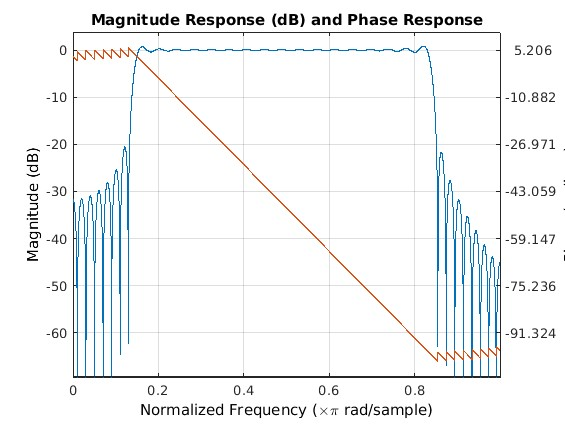
\includegraphics[width=1.5\linewidth, height=0.65\textheight]{bandpass_freq.jpg}
    \label{fig:my_label}
\end{figure}

\subsection{Magnitude Response}
\begin{figure}[H]
\hspace*{-2.5cm}
    \centering
    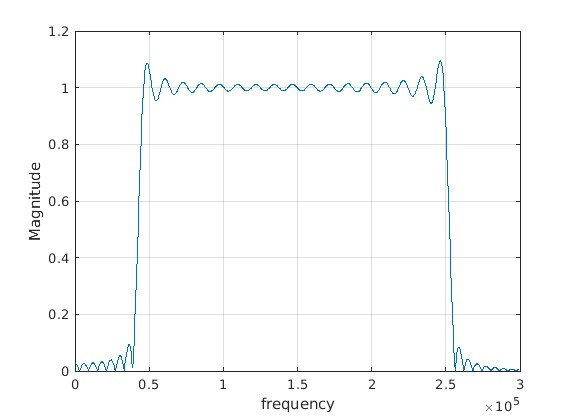
\includegraphics[width=1.5\linewidth, height=0.65\textheight]{Bandpass_mag.jpg}
    \label{fig:my_label}
\end{figure}

\subsection{Impulse Response}
\begin{figure}[H]
\hspace*{-2.5cm}
    \centering
    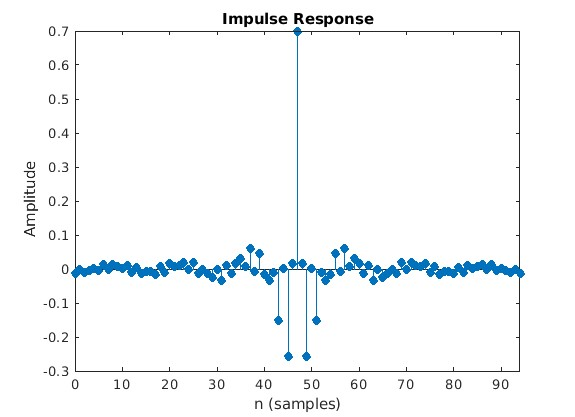
\includegraphics[width=1.5\linewidth, height=0.65\textheight]{IR_BP.jpg}
    \label{fig:my_label}
\end{figure}

\subsection{Coefficients}
\begin{figure}[H]
\hspace*{-2.5cm}
    \centering
    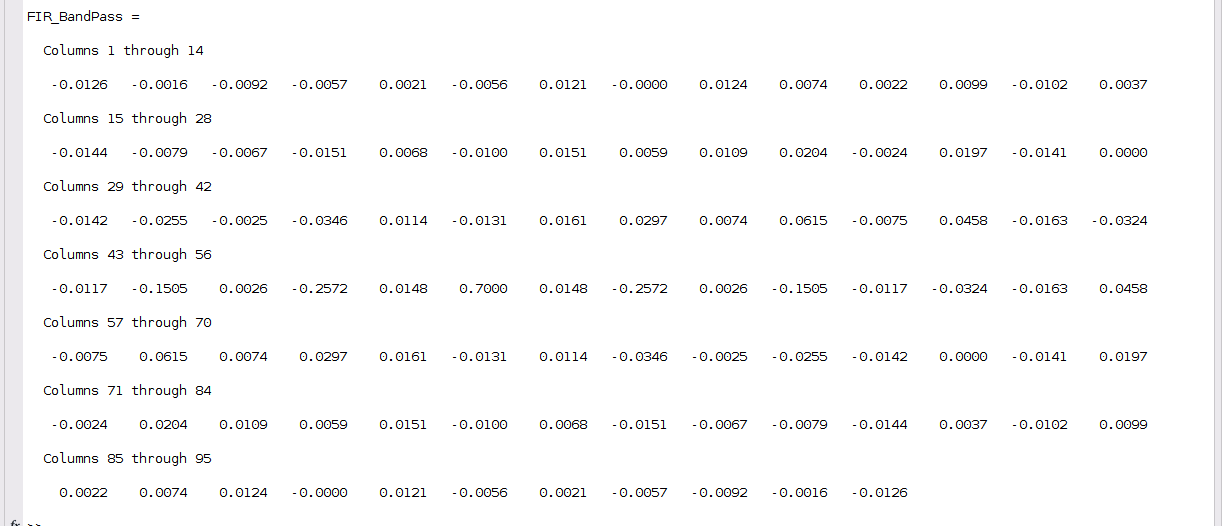
\includegraphics[width=1.5\linewidth, height=0.55\textheight]{coeff_BP.png}
    \label{fig:my_label}
\end{figure}


\newpage
\section{\textbf{Bandstop Filter}}
\subsection{\textbf{Un-normalized Discrete Time Filter Specifications}}

\vspace{1.5em}
\noindent
The specifications of this filter are :
\begin{itemize}
    \item Stopband : \textbf{80 - 215 KHz}
    \item Passband : \textbf{0 - 75 KHz} and \textbf{220 - 300 KHz}
    \item  Transition band : \textbf{5KHz} on either side of passband
    \item  Tolerance : \textbf{0.15} in \textbf{magnitude} for both passband and stopband
\end{itemize}

\subsection{Normalized Digital Filter Specifications}
Sampling rate = 600KHz\\
In the normalized frequency axis, sampling rate corresponds to 2$\pi$\\
Therefore, any frequency can be normalized as follows :
\begin{equation*}
    \omega = \frac{\Omega*2\pi}{\Omega_s}
\end{equation*}
where $\Omega_s$ is the Sampling Rate.\\

\vspace{1em}
\noindent
For the normalized discrete filter specifications, the nature and tolerances being the dependent variables remain the same while the passband and stopband frequencies change as per the above transformations. 
\begin{itemize}
    \item Stopband : \textbf{0.267 - 0.717} {$\pi$}
    \item Passband : \textbf{0 -  0.25} {$\pi$} and \textbf{0.733 - 1} {$\pi$}
    \item  Transition band : \textbf{0.0167} $\pi$ on either side of stopband
\end{itemize}

\section{FIR Bandstop Filter}

Both the passband and stopband tolerances are given to be 0.15\\
Therefore $\delta$ = 0.15 and the minimum stopband attenuation A is given by :
\begin{equation*}
    A = -20log(\delta) = -20log(0.15) = 16.478 
\end{equation*}
Since A $<$ 21, we get $\beta$ = 0, where $\beta$ is the shape parameter of Kaiser window
Now to estimate the window length required, we use the empirical formula for the lower bound on
the window length

\begin{equation*}
    2N_{min} + 1 \geq 1+ \frac{A - 7.95}{2.285*\Delta \omega_T}
\end{equation*}\

Here $\Delta \omega_T$ is the transition width which is the same on either side of the passband
\begin{equation*}
    \Delta \omega_T = \frac{5KHz*2 \pi}{600KHz} = 0.0167 \pi
\end{equation*}
\begin{equation*}
    2N_{min} \geq 71.279 
\end{equation*}
Hence we initially choose $N_{min}$ = 36 ( $N_{min}$ is such that total number of samples is 2$N_{min}$+1) Further for stringent tolerance and transition band specifications, we get $N_{total}$ = 2$N_{min}$ + 23 = 95  using trial and error.\\

The time domain coefficients were obtained by first generating the ideal impulse response samples
for the same length as that of the window. The Kaiser Window was generated using the MATLAB
function and applied on the ideal impulse response samples. For generating the ideal impulse response a separate function was made to generate the impulse response of Low-Pass filter. It took the cutoff value and the number of samples as input argument. The band-stop impulse response samples were generated as the difference between an all pass filter and a band pass filter such that the cutoff frequencies are again at average of passband and stopband frequencies i.e. 0.2583 $\pi$ and 0.725 $\pi$


\section{Matlab Plots}
\subsection{Frequency Response}
\begin{figure}[H]
\hspace*{-2.5cm}
    \centering
    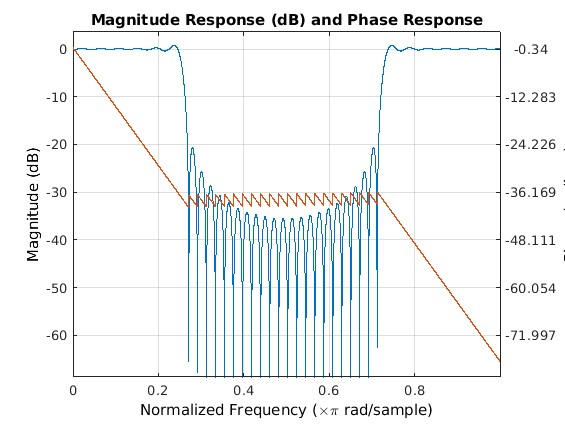
\includegraphics[width=1.5\linewidth, height=0.65\textheight]{bandstop_freq.jpg}
    \label{fig:my_label}
\end{figure}

\subsection{Magnitude}
\begin{figure}[H]
\hspace*{-4cm}
    \centering
    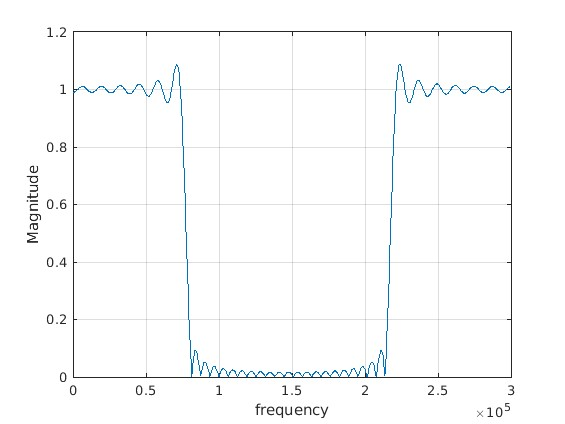
\includegraphics[width=1.6\linewidth, height=0.65\textheight]{bandstop_mag.jpg}
    \label{fig:my_label}
\end{figure}

\subsection{Impulse Response}
\begin{figure}[H]
\hspace*{-2.5cm}
    \centering
    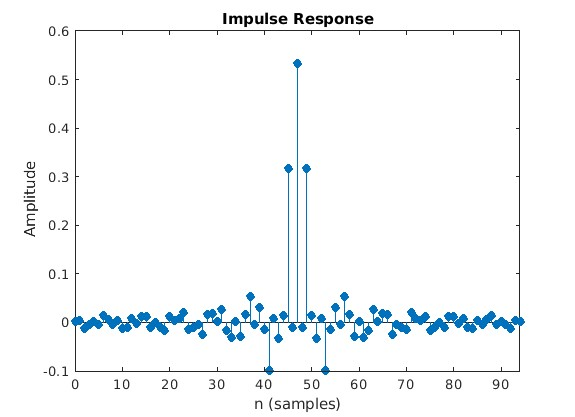
\includegraphics[width=1.5\linewidth, height=0.6\textheight]{IR_BS.jpg}
    \label{fig:my_label}
\end{figure}

\subsection{Coefficients}
\begin{figure}[H]
\hspace*{-2.5cm}
    \centering
    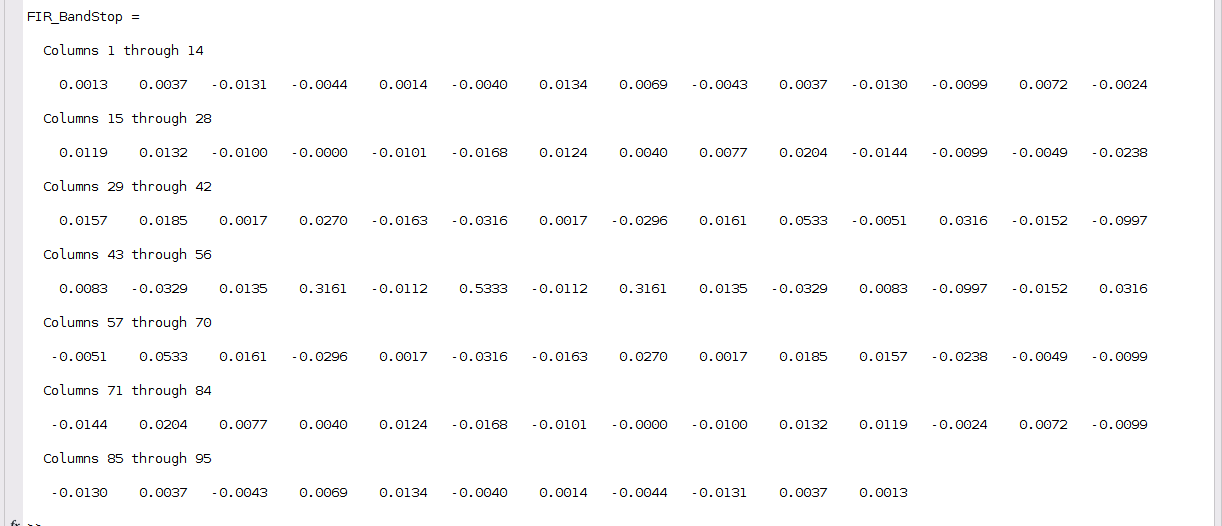
\includegraphics[width=1.5\linewidth, height=0.55\textheight]{coeff_BS.png}
    \label{fig:my_label}
\end{figure}

\section{Final results after cascading the two filters}

\section{Matlab Plots}
\subsection{Frequency Response}
\begin{figure}[H]
\hspace*{-2.5cm}
    \centering
    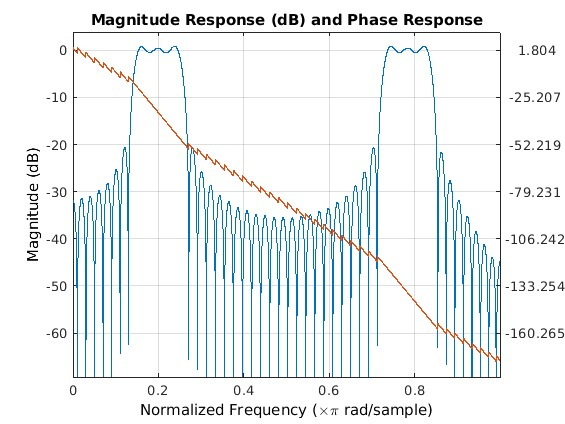
\includegraphics[width=1.5\linewidth, height=0.65\textheight]{Multiband_freq.jpg}
    \label{fig:my_label}
\end{figure}

\subsection{Magnitude}
\begin{figure}[H]
\hspace*{-4cm}
    \centering
    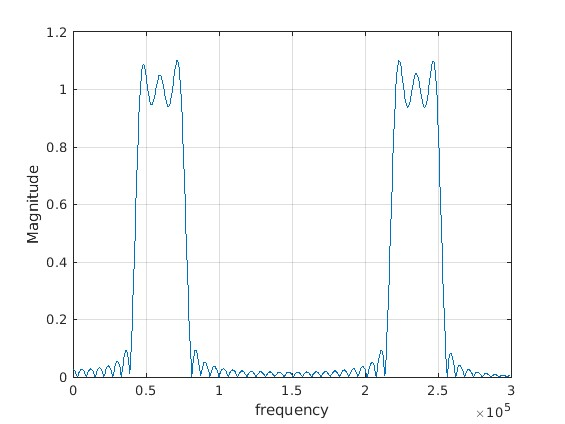
\includegraphics[width=1.6\linewidth, height=0.65\textheight]{Multiband_mag.jpg}
    \label{fig:my_label}
\end{figure}

\subsection{Impulse Response}
\begin{figure}[H]
\hspace*{-2.5cm}
    \centering
    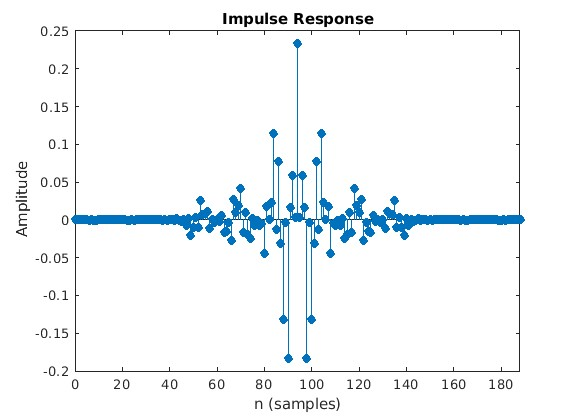
\includegraphics[width=1.5\linewidth, height=0.6\textheight]{IR_multiband.jpg}
    \label{fig:my_label}
\end{figure}

\subsection{Coefficients}
\begin{figure}[H]
\hspace*{-2.5cm}
    \centering
    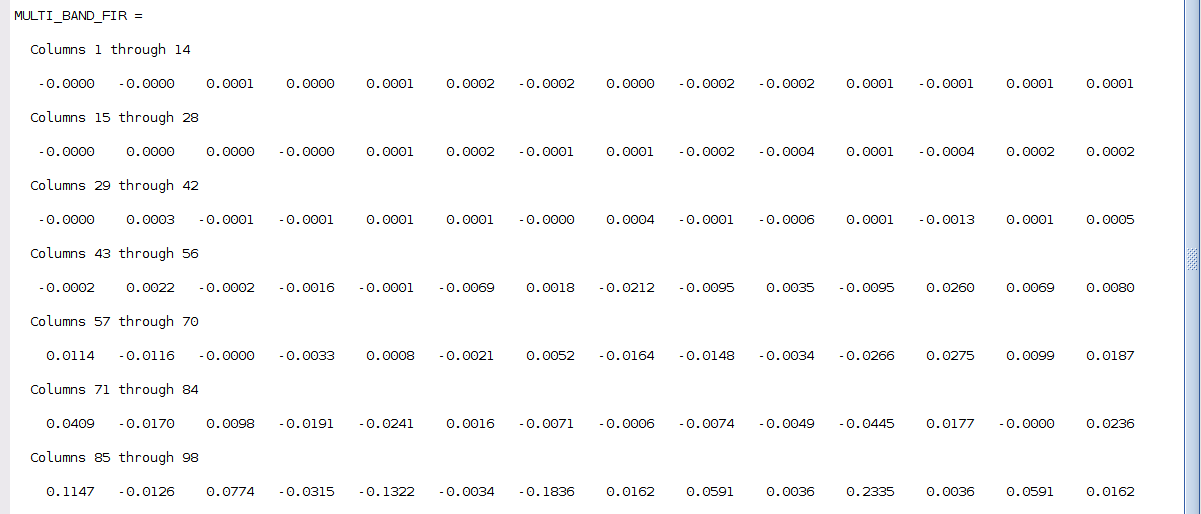
\includegraphics[width=1.5\linewidth, height=0.55\textheight]{multiband1.png}
    \label{fig:my_label}
\end{figure}

\begin{figure}[H]
    \hspace*{-2.5cm}
        \centering
        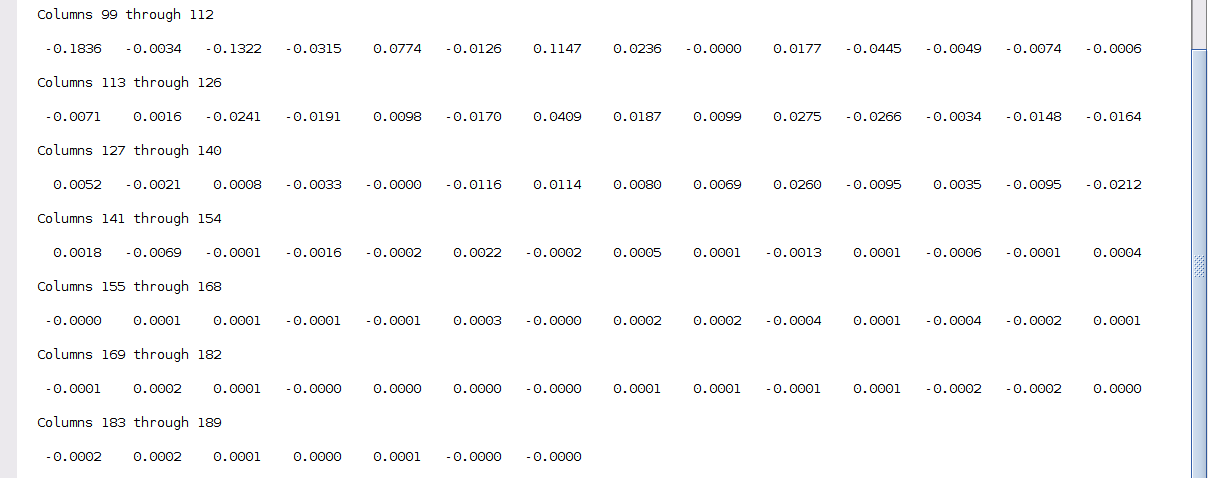
\includegraphics[width=1.5\linewidth, height=0.55\textheight]{multiband2.png}
        \label{fig:my_label}
    \end{figure}

\section{Comparison between FIR and IIR Filters :}
\begin{itemize}
    \item FIR filters are easier to design as we only need to truncate the ideal impulse response using a suitable window function, instead of applying the bilinear and frequency transformation, designing a low-pass filter and then converting it to bandpass/bandstop as per our requirement.
    \item We get a linear (or psuedo linear) phase response in FIR Filter which we don't get in IIR Filters.
    \item We can't control the passband and stopband tolerances individually in FIR Filters, nor can we change their nature (monotonic or equiripple), which was possible in IIR Filters.
    \item We usually need a lot more resources for FIR filters as compared to IIR
    filters, as we can see that the value of N for FIR filters is considerably
    large.
\end{itemize}
\section{Review}

\begin{itemize}
    \item I have verified the filter design of my team-mate Tamojeet Roychowdhury (Roll No : 21D070079) 
\end{itemize}
\end{document}
